\documentclass[10pt, t]{beamer}
\usetheme{metropolis}           % Use metropolis theme

\ifnotes
  \hypersetup{final}
  \usepackage{pgfpages}
  \setbeamertemplate{note page}[plain]
  \setbeameroption{show notes on second screen=right}
  % the following fixes bug which causes normal text to be white instead of
  % template default when notes are enabled
  % (see https://tex.stackexchange.com/questions/232168/normal-text-is-invisible-when-using-beamer-with-notes-and-xelatex)
  \makeatletter 
  \def\beamer@framenotesbegin{% at beginning of slide
       \usebeamercolor[fg]{normal text}
        \gdef\beamer@noteitems{}% 
        \gdef\beamer@notes{}% 
  }
  \makeatother
\fi

\usepackage{appendixnumberbeamer}
\usepackage{algpseudocode}
\usepackage{multirow}
\usepackage{verbatim}
\usepackage{tikz}
\usetikzlibrary{decorations.pathreplacing}
\usepackage[scale=3]{ccicons}   % creative commons icons

\title{Parallel algorithm design}
\date{}
\author{Jeremy Iverson}
\institute{College of Saint Benedict \& Saint John's University}

\begin{document}

  \begin{frame}
    \titlepage
  \end{frame}

  \begin{frame}{Parallel algorithm design}
    \begin{itemize}
      \item how do we identify concurrency in our algorithms?
      \item how do we assign work to processes?
      \item how do we distribute data to processes?
    \end{itemize}

    \note[item] {all of these things affect our analysis --- potentially
      introducing parallel overhead and decreasing speedup}
  \end{frame}

  \begin{frame}{Problem decomposition}
    \begin{itemize}
      \item the process of dividing the computation into smaller pieces of work,
        i.e., \emph{tasks}
      \item tasks are programmer defined
    \end{itemize}

    \note[item] {answers questions of how do we identify concurrency in our
      algorithms}
  \end{frame}

  \begin{frame}{Example --- dense matrix-multiplication}
    \note[item] {show this example on the board}
    \note[item] {just point out what we defined as tasks, and ask why? ---
      because it was the easiest / most natural?}
    \note[item] {are there any other ways that we could have decomposed the
      problem?}
  \end{frame}

  \begin{frame}{Example --- query processing}
    \begin{center}
      \small
      \begin{tabular}{clrlcc}
        \hline
        ID\# & Model   & Year & Color & Dealer & Price \\
        \hline
        4523 & Civic   & 2002 & Blue  & MN     & \$18,000 \\
        3476 & Corolla & 1999 & White & IL     & \$15,000 \\
        7623 & Camry   & 2001 & Green & NY     & \$21,000 \\
        9834 & Prius   & 2001 & Green & CA     & \$18,000 \\
        6734 & Civic   & 2001 & White & OR     & \$17,000 \\
        5342 & Altima  & 2001 & Green & FL     & \$19,000 \\
        3845 & Maxima  & 2001 & Blue  & NY     & \$22,000 \\
        8354 & Accord  & 2000 & Green & VT     & \$18,000 \\
        4395 & Civic   & 2001 & Red   & CA     & \$17,000 \\
        7352 & Civic   & 2002 & Red   & WA     & \$18,000 \\
        \hline
        \multicolumn{6}{r}{\tiny{\href{https://www.pearson.com/us/higher-education/program/Grama-Introduction-to-Parallel-Computing-2nd-Edition/PGM11645.html}{A database storing information about used vehicles.}}}
      \end{tabular}
    \end{center}

    \small
    \fbox{MODEL=``Civic'' AND YEAR=``2001'' AND (COLOR=``Green'' OR COLOR=``White'')}

    \note[item] {relation database of vehicles}
    \note[item] {query looks for all 2001 Civics whose color is either Green or
      White}
    \note[item] {in a relational database, this query could be processed by
      creating a number of intermediate tables}
    \note[item] {the intermediate tables are combined using set intersection /
      union}
  \end{frame}

  \begin{frame}{Example --- query processing cont'd}
    \vspace{-3ex}
    \begin{center}
      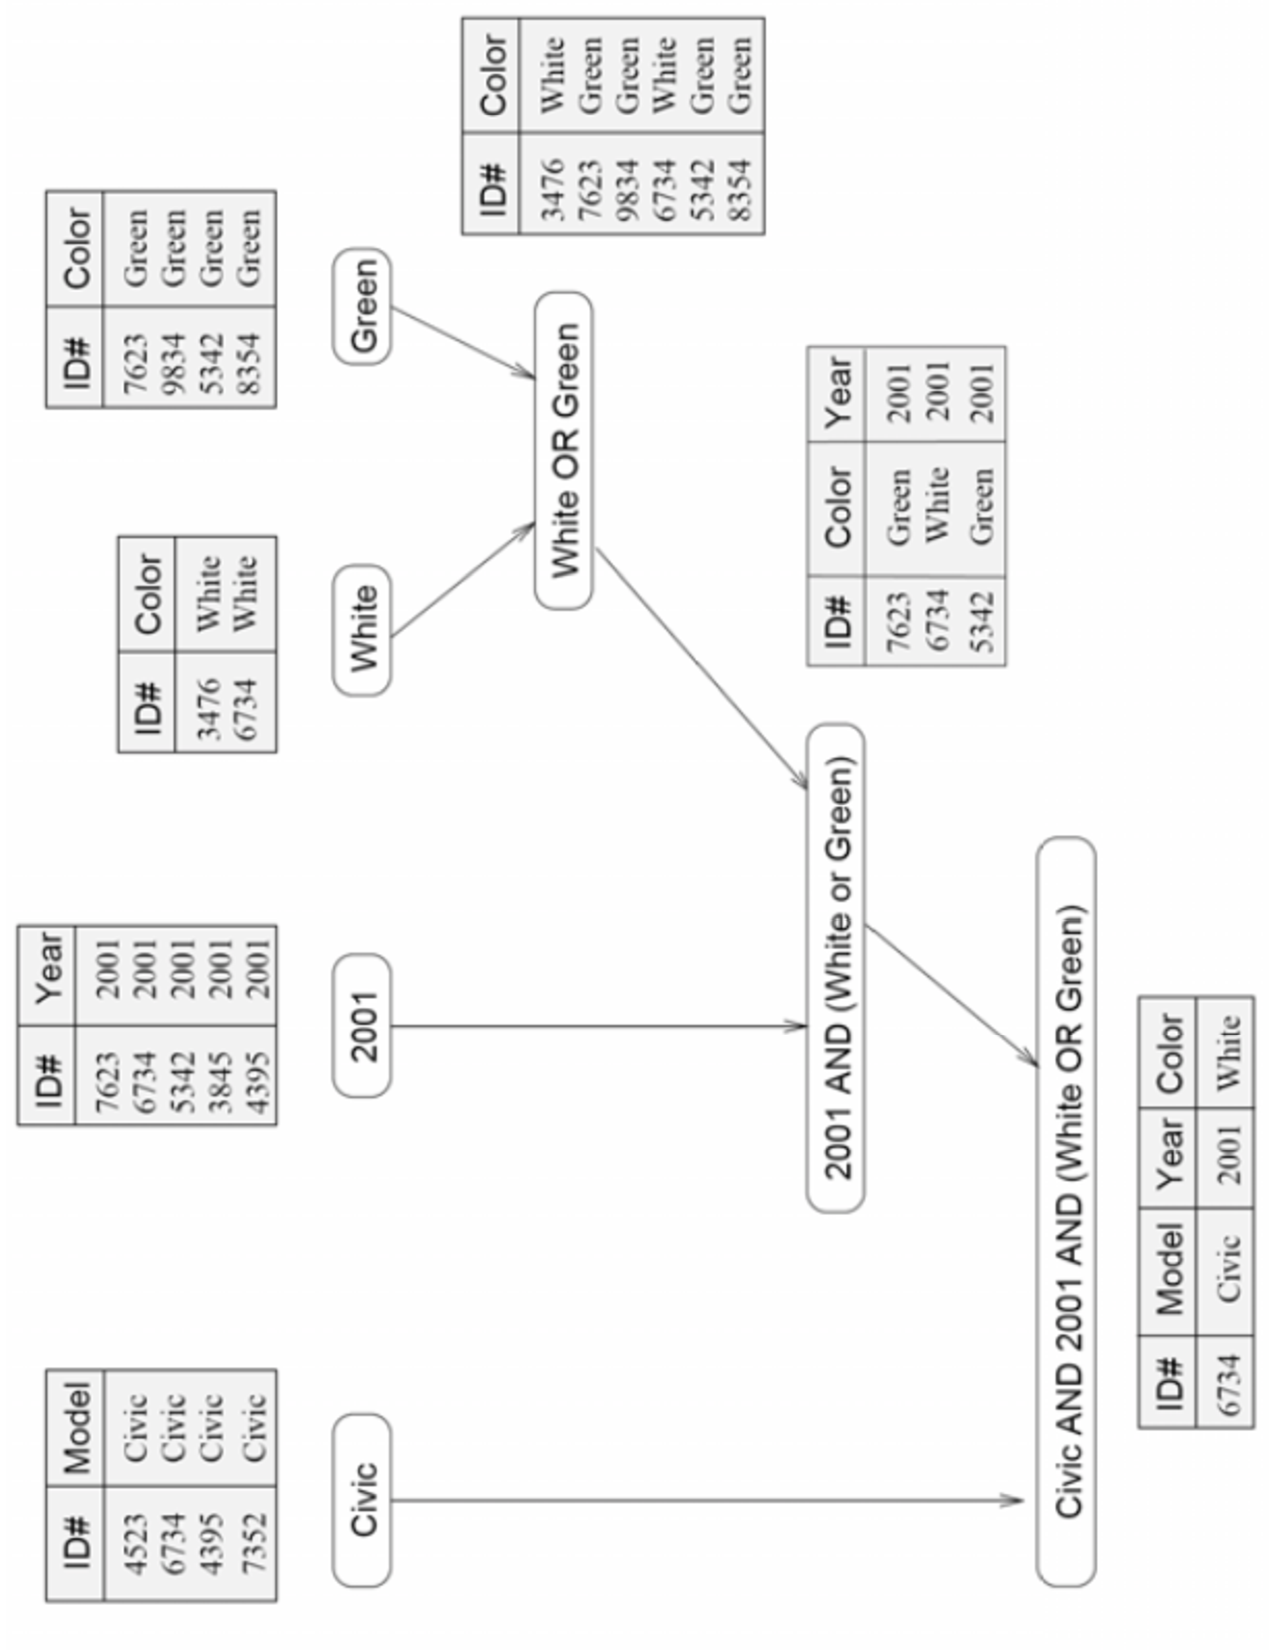
\includegraphics[angle=-90,width=.80\textwidth]{query2}\\
      \hfill\tiny{\href{https://www.pearson.com/us/higher-education/program/Grama-Introduction-to-Parallel-Computing-2nd-Edition/PGM11645.html}{The different tables and their dependencies in a query processing operation.}}
    \end{center}

    \note[item] {the task dependency graphs for a serialized way of organizing
      the computations}
  \end{frame}

  \begin{frame}<1>[label=queryprocessing]{Example --- query processing\only<1>{ cont'd}}
    \vspace{-3ex}
    \begin{center}
      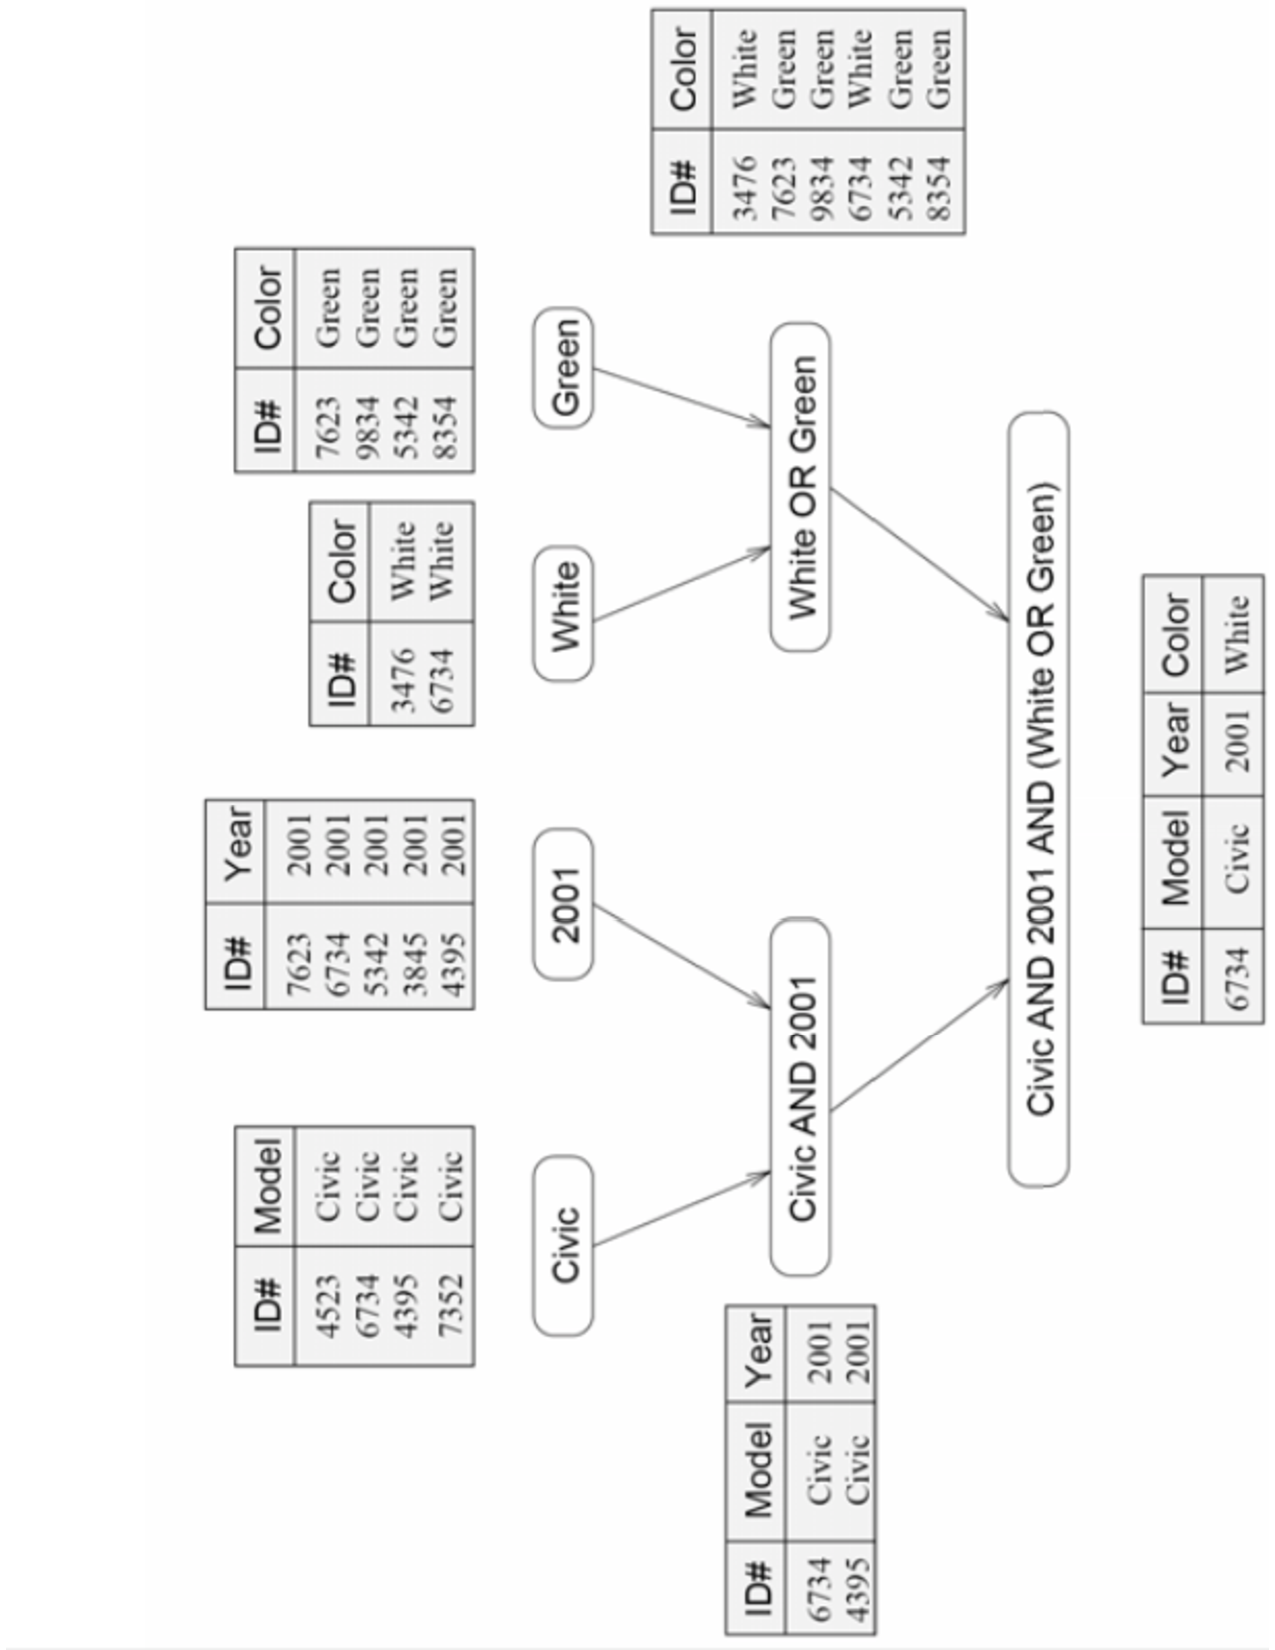
\includegraphics[angle=-90,width=.80\textwidth]{query1}\\
      \hfill\tiny{\href{https://www.pearson.com/us/higher-education/program/Grama-Introduction-to-Parallel-Computing-2nd-Edition/PGM11645.html}{The different tables and their dependencies in a query processing operation.}}
    \end{center}

    \note<1>[item] {an organization that exposes more concurrency}
    \note<2>[item] {what sort of decomposition is this?}
  \end{frame}

  \begin{frame}{Task-dependency graph}
    \begin{itemize}
      \item represented using a directed acyclic graph (DAG)
    \end{itemize}
    \vspace{-10ex}
    \begin{center}
      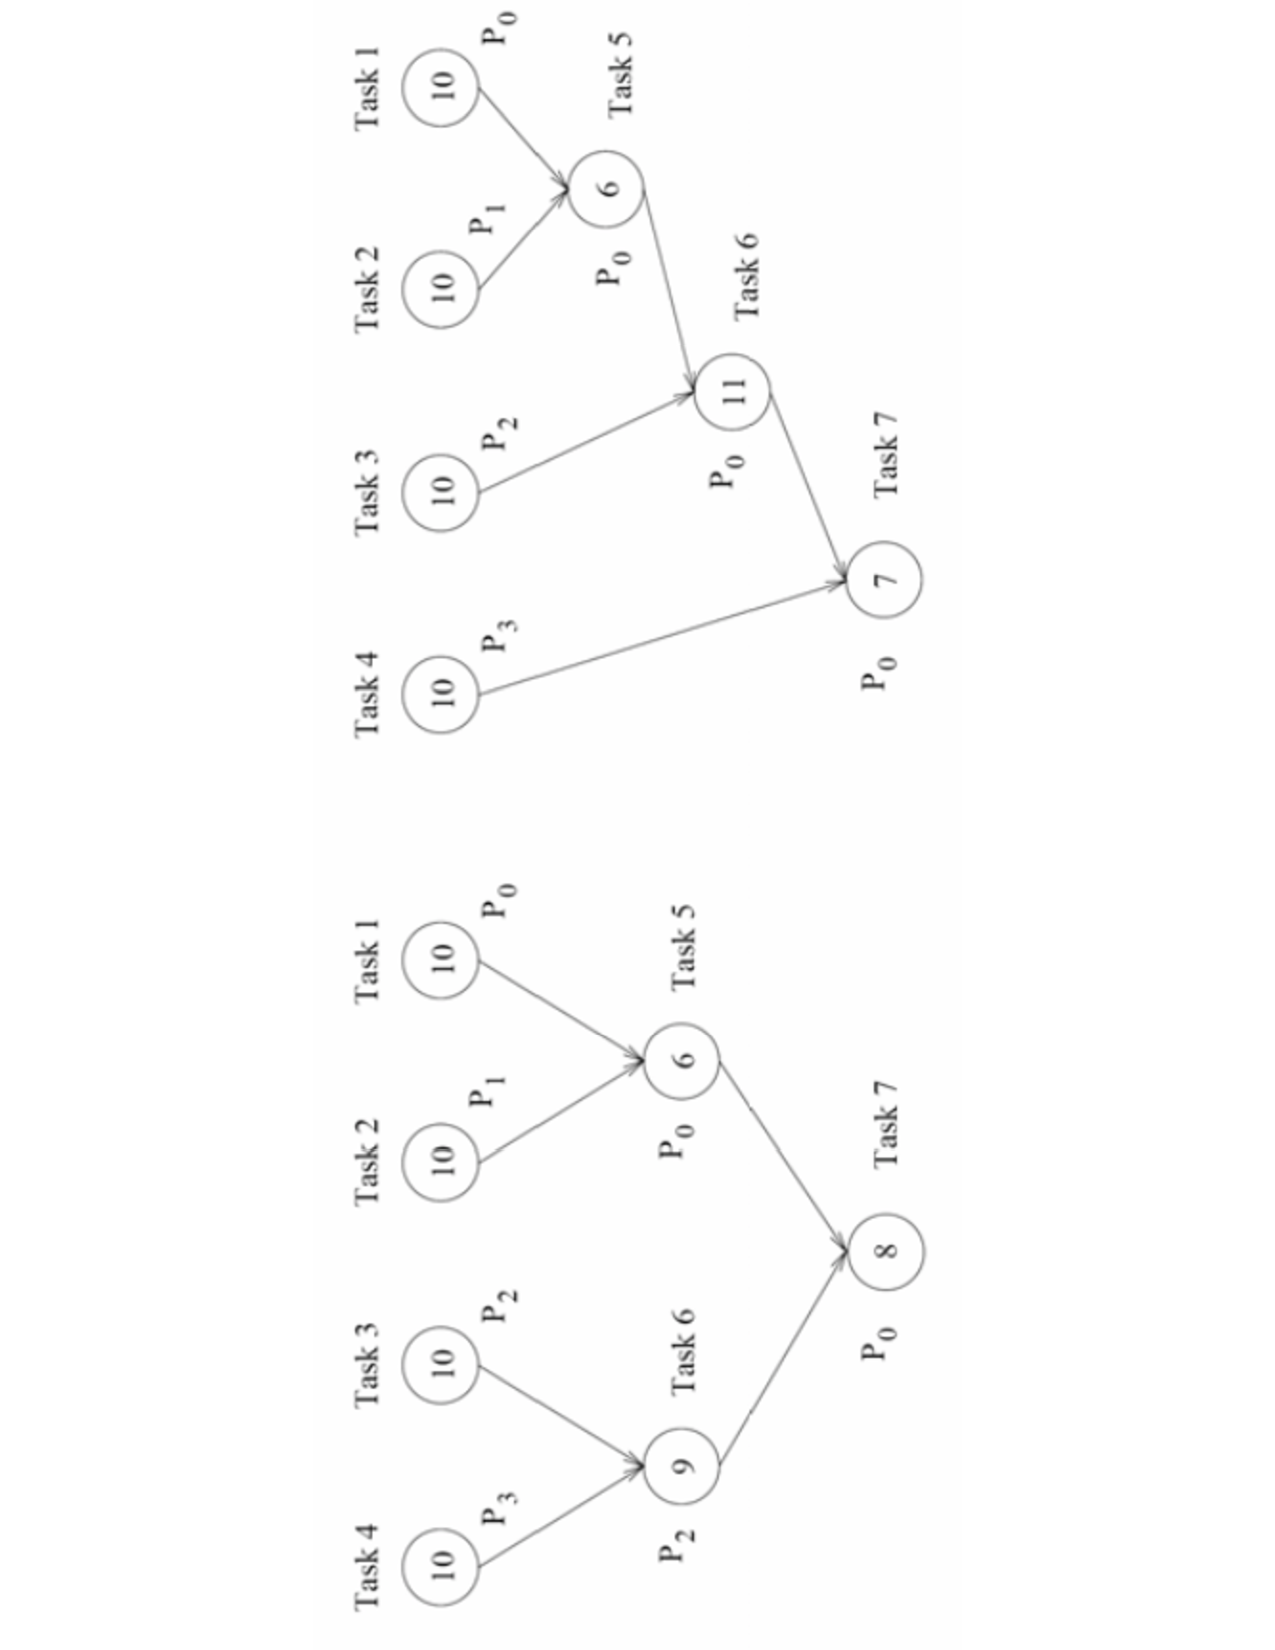
\includegraphics[angle=-90,width=.80\textwidth]{query-dag}\\
      \vspace{-8.5ex}
      \hfill\tiny{\href{https://www.pearson.com/us/higher-education/program/Grama-Introduction-to-Parallel-Computing-2nd-Edition/PGM11645.html}{Task-dependency graphs and their mappings onto four processes for query processing.}}
    \end{center}

    \begin{block}{useful metrics}
      \begin{itemize}
        \item degree of concurrency
        \item critical path
      \end{itemize}
    \end{block}

    \note[item] {degree of concurrency --- the number of tasks that can be
      executed concurrently}
    \note[item] {critical path --- sum of the weights of nodes along the
      longest directed path between any pair of start and finish nodes}
    \note[item] {the ratio of critical path to total work is the average
      degree of concurrency --- in this example 63/27=2.33 and 64/34=1.88
      respectively}
    \note[item] {what is the relationship between critical path and other
      metrics that we have studied?}
  \end{frame}

  \begin{frame}{Common decomposition methods}
    \begin{itemize}
      \item data decomposition
      \item recursive decomposition
      \item exploratory decomposition
      \item speculative decomposition
      \item hybrid decomposition
    \end{itemize}

    \note[item] {up until now, our technique for identifying tasks was pretty
      adhoc, i.e., based on our expert experience, not a programmatic approach}
    \note[item] {we will focus mostly on data decomposition --- it is the most
      common}
  \end{frame}

  \begin{frame}{Data decomposition}
    \begin{itemize}
      \item derive the tasks by focusing on the multiplicity of the data
      \item consists of two steps:
        \begin{enumerate}
          \item partition the data
          \item derive tasks from the data partitioning
        \end{enumerate}
      \item common data decompositions
        \begin{itemize}
          \item input
          \item output
          \item intermediate
        \end{itemize}
      \item owner computes rule
    \end{itemize}

    \note[item] {how to derive tasks from data partitioning? --- owner computes
      rule}
    \note[item] {owner computes rule --- tasks are all computations associated
      with a partition of data}
  \end{frame}

  \begin{frame}{Input decomposition}
    \note[item] {matrix-multiplication on board}
  \end{frame}

  \begin{frame}{Output decomposition}
    \note[item] {matrix-multiplication on board}
  \end{frame}

  \againframe<2>{queryprocessing}

  \begin{frame}{Intermediate decomposition}
    coming soon\dots
  \end{frame}

  %\begin{frame}[standout]
  %  \ifnotes
  %    \usebeamercolor[white]{normal text} % override bug fix in preamble
  %  \fi
  %\end{frame}

  \appendix

  \begin{frame}[c]
    \begin{center}\ccbysa\end{center}

    except where otherwise noted, this worked is licensed under
    \href{http://creativecommons.org/licenses/by-sa/4.0/}{creative commons
    attribution-sharealike 4.0 international license}
  \end{frame}
\end{document}
